\documentclass[toc=bib]{scrartcl}
\title{Simplicial Homology}
\author{Jan Zwank}
\usepackage{amsmath,amssymb,amsthm}
\usepackage[utf8]{inputenc}
\usepackage[T1]{fontenc}
\usepackage{hyperref,microtype,lmodern,csquotes}
\usepackage[english]{babel}
\usepackage{tikz, tikz-cd}
\usetikzlibrary{3d,calc,decorations}
\usepackage{pst-solides3d}
\usepackage{caption}
\usepackage{array}

\theoremstyle{plain}
\newtheorem{theorem}{Theorem}[section]
\newtheorem{lemma}[theorem]{Lemma}
\newtheorem{korollar}[theorem]{Korollar}
\newtheorem{satz}[theorem]{Satz}
\newtheorem{hilfssatz}[theorem]{Hilfssatz}
\newtheorem{corollary}[theorem]{Corollary}

\theoremstyle{definition}
\newtheorem	{definition}[theorem]{Definition}
\newtheorem{beispiel}[theorem]{Beispiel}
\newtheorem{beispiele}[theorem]{Beispiele}
\newtheorem{konvention}[theorem]{Konvention}
\newtheorem{notation}[theorem]{Notation}
\newtheorem{axiom}[theorem]{Axiom}
\newtheorem{example}[theorem]{Example}
\newtheorem{examples}[theorem]{Examples}

\theoremstyle{remark}
\newtheorem*{bemerkung}{Bemerkung}
\newtheorem*{bemerkungen}{Bemerkungen}
\newtheorem*{frage}{Frage}

\usetikzlibrary{decorations.markings,intersections}
\tikzset{->-/.style={decoration={
			markings,
			mark=at position #1 with {\arrow[line width=3pt]{stealth}}},postaction={decorate}}}

\newcommand{\Bd}{\mathrm{Bd}\,}
\newcommand{\Int}{\mathrm{Int}\,}
\newcommand{\pprime}{{\prime\prime}}
\newcommand{\ppprime}{{\pprime\prime}}
\newcommand{\isom}{\cong}
\newcommand{\SH}{Simplicial Homology}
\newcommand{\sh}{simplicial homology}
\newcommand{\Z}{\mathbb{Z}}
\newcommand{\Sp}{\mathbb{S}}
\newcommand{\im}{\mathrm{Im}\,}
\newcommand{\qandq}{\quad \text{and} \quad}
\newcommand{\qqandqq}{\qquad \text{and} \qquad}
\newcommand{\scs}{simplicial complexes}
\usepackage%[style=authoryear]
	{biblatex}
\bibliography{bibliography}
\begin{document}
	\maketitle
	
	\begin{abstract}
		\textsc{Abstract.}\textit{
		Simplicial homology is a valuable tool for distinguishing polyhedra. We achieve that by assigning an abelian groups $H_n(X;G)$ to the underlying simplicial complex of the polyhedron $|X|$. We call these groups the Homology groups of $X$ with coefficients in $G$, where $G$ is an abelian Group. As we will see, simplicial homology is in fact a functor from the category of simplicial complexes to the category of abelian groups. In addition, we will see that Homology groups only depend on the homotopy type, i.e. two spaces that are homotopy equivalent have isomorphic Homology groups.
		}
	\end{abstract}
\clearpage
\tableofcontents

\clearpage

\section{Motivation}\label{motivation}
One of the main goals when studying (topological) spaces (or in this case \scs) is to determine whether two spaces are homeomorphic or at least homotopy equivalent (see Definition \ref{def:hom-eq}) 
or not. The first approach would be to check if both spaces are simply connected. A more advanced method checks if the fundamental groups $\pi_1$ coincide\footnote{The fundamental group $\pi_1(X)$ is the group of all closed paths with the group action being concatenation. If $X$ is a simply connected space then $\pi_1(X)=0$. Furthermore, the fundamental group is homotopy invariant (up to isomorphism), so homotopic spaces have isomorphic fundamental groups. A more precise formulation of this statement can be found in Hatchers book \parencite[Prop. 1.18, p. 37]{ha}:
\begin{quotation}
	\begin{quote}
		If $\phi: X\to Y$ is a homotopy equivalence, then the induces homomorphism $\phi_*:\pi_1(X,x_0)\to\pi_1(Y,\phi(x_0))$ is an isomorphism for all $x_0\in X$.
	\end{quote}
\end{quotation} }.

It turns out that this is a valuable tool for one and two dimensional \scs. But this method fails for complexes with higher dimensional simplices. For example $\pi_1(\mathbb{S}^n)=0$ for all $n\geq 2$. It is therefore impossible to show that two spheres of dimension greater or equal 2 are only then homeomorphic if they are of the same dimension. It can be shown that the fundamental group actually only depends on the 2-skeleton of the complex \cite[vgl.][p. 173]{ar}. 

Even though this method can be generalized to the study of higher homotopy groups $\pi_n$, this is often more difficult than necessary since the computation of those groups is far from trivial.

In the following we will explore the concept of \sh{} groups and how it can be used to classify spaces. We will see that they allow us to tackle the problem of deciding whether two \textbf{polyhedra}\footnote{A polyhedron is the polytope of a simplicial complex.} are homeomorphic. Note that isomorphic Homology classes do not automatically mean that the spaces are homeomorphic. In fact the torus $T$ and $\mathbb{S}^1\wedge\mathbb{S}^1$ have the same homology groups in every dimension but they are not homeomorphic ($\pi_1(T)=\Z\oplus\Z$ whereas $\pi_1(\mathbb{S}^1\wedge\mathbb{S}^1)=\Z\ast\Z$) .

It is possible to extend the concept of Homology to more general spaces than polyhedra using singular homology, however those will not be covered here. The interested reader might refer to the book of Munkres \cite{mu} or Hatcher \cite{ha} to learn more about singular homology groups.

While we considered all possible paths when we were talking about the fundamental group we will now only consider those that aren't the boundary of a portion of the surface. A great motivation for this approach is given by Armstrong \cite[p. 173f]{ar}:

When we concern ourselves with the question how closed paths on the torus are different from those on the sphere, we can notice the following:
Any Jordan curve (i.e. nonselfintersecting, closed path) on a sphere divides the surface into two \glqq regions\grqq{} as depicted in \autoref{divided-sphere}\footnote{For a more precise statement see \url{https://en.wikipedia.org/wiki/Jordan_curve_theorem}}. The same is not true for the torus. In \autoref{path-on-torus} we see that even tough there are Jordan curves on a torus that bound a \glqq region\grqq of the surface, not all Jordan curves have that property \cite[see][p. 173f]{ar}.



%Any closed path on the 2-sphere divides the surface into two regions as shown in \autoref{divided-sphere}\footnote{For a more precise statement see \url{https://en.wikipedia.org/wiki/Jordan_curve_theorem}}.

\begin{figure}[h]
	
\parbox{\linewidth}{\parbox[t]{.5\linewidth}{\centering
	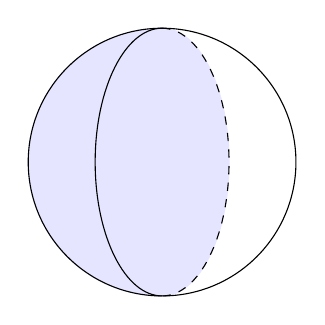
\begin{tikzpicture}[scale=1.7]
		%\draw (-1,0) arc (180:360:1cm and 0.5cm);
		%\draw[dashed] (-1,0) arc (180:0:1cm and 0.5cm);
		\filldraw[blue!10] (0,1)  arc (90:270:1cm) arc (-90:90:0.5cm and 1cm);
		\draw (0,1) arc (90:270:0.5cm and 1cm);
		\draw[dashed] (0,1) arc (90:-90:0.5cm and 1cm);
		\draw (0,0) circle (1cm);
		%\shade[ball color=blue!10!white,opacity=0.20] (0,0) circle (1cm);
	\end{tikzpicture}}%
\parbox[t]{.5\linewidth}{\centering
	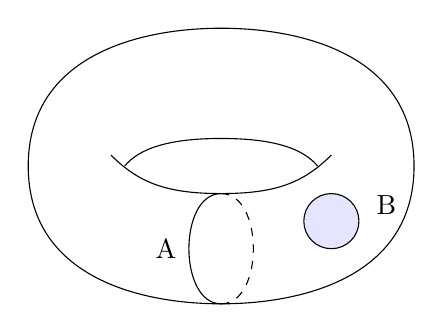
\begin{tikzpicture}[scale=0.7]
	\draw (-3.5,0) .. controls (-3.5,2) and (-1.5,2.5) .. (0,2.5);
	\draw[xscale=-1] (-3.5,0) .. controls (-3.5,2) and (-1.5,2.5) .. (0,2.5);
	\draw[rotate=180] (-3.5,0) .. controls (-3.5,2) and (-1.5,2.5) .. (0,2.5);
	\draw[yscale=-1] (-3.5,0) .. controls (-3.5,2) and (-1.5,2.5) .. (0,2.5);
	
	\draw (-2,.2) .. controls (-1.5,-0.3) and (-1,-0.5) .. (0,-.5) .. controls (1,-0.5) and (1.5,-0.3) .. (2,0.2);
	
	\draw (-1.75,0) .. controls (-1.5,0.3) and (-1,0.5) .. (0,.5) .. controls (1,0.5) and (1.5,0.3) .. (1.75,0);
	
	\draw (0,-0.5) to [out=180, in=180](0,-2.5);
	\draw[dashed] (0,-2.5) to [out=0, in=0](0,-0.5);
	\draw (-1,-1.5) node{A};
	\draw[fill=blue!10!white] (2,-1) circle (0.5);
	\draw (3,-.7) node{B};
	\end{tikzpicture}
%\begin{pspicture}(-6,-4)(6,4)
%\psset{viewpoint=30 0 15 rtp2xyz,Decran=30,lightsrc=viewpoint}
%\psSolid[object=tore,r1=2.5,r0=.7,ngrid=36 72,fillcolor=blue!10!white,grid=false]%
%\end{pspicture}
}}
\parbox[t]{.5\linewidth}{\captionsetup{width=.9\linewidth}
\caption{Any closed path on the sphere divides the surface into two regions.\label{divided-sphere} }}%
\parbox[t]{.5\linewidth}{\captionsetup{width=.9\linewidth}
\caption{There are closed paths on the torus that do not divide the surface into two regions.\label{path-on-torus}}}

\end{figure}

\section{\SH{} Groups with Integer Coefficients}\label{first-hom}

Before we get started, let us remind ourselves of some definitions and notations as can be found in Munkres' book \cite[p. 26f.]{mu}
\begin{definition}
	For a simplex $\sigma$ we say that two orderings of its vertex set are equivalent if they differ by an even permutation. For a simplex with nonzero dimension, the orderings of the vertices fall into two equivalence classes, called the \textbf{orientations} of $\sigma$. An \textbf{oriented simplex} is a simplex together with an orientation.
\end{definition}
Further we will use the same notation as Munkres \cite[p. 26]{mu}
\begin{notation}
	For geometrically independent points $v_0,\dots,v_p$ we denote the simplex they span with
	\[
	[v_0,\dots,v_p].
	\]
	For an oriented simplex we will use the notation
	\[
	(v_0,\dots,v_p).
	\]
	where the orientation is given by this particular ordering.
%	A change in orientation will be denoted by a minus sign. So, for example
%	\[
%	(v_1,v_2,v_3)=(v_2,v_3,v_1)=(v_3,v_1,v_2)=-(v_1,v_3,v_2)=-(v_2,v_1,v_3)=-(v_3,v_2,v_1)
%	\]
\end{notation}

A choice of orientation is usually depicted with arrows as can be seen in \autoref{orientation-arrows}

\begin{figure}
	\centering

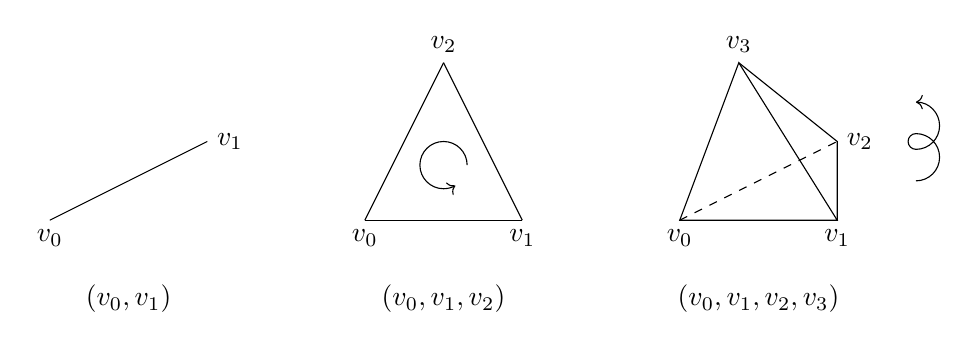
\begin{tikzpicture}
	\draw[] (0,0) node[below]{$v_0$}->(1,0.5);
	\draw (1,0.5)-- (2,1) node[right]{$v_1$};
	\draw (1,-1) node{$(v_0,v_1)$};
	%
	\draw[] (4,0) node[below]{$v_0$}--(6,0)node[below]{$v_1$};
	\draw[] (6,0) -- (5,2) node[above]{$v_2$};
	\draw[] (5,2)--(4,0);
	\draw (5,-1) node{$(v_0,v_1,v_2)$};	
	\draw[->] (5.3,0.7)arc[start angle=0, end angle=300,radius=0.3cm];
	%
	\draw (8,0) node[below]{$v_0$}--(10,0)node[below]{$v_1$}--(8.75,2)node[above]{$v_3$}--cycle;
	\draw (10,0)--(10,1)node[right]{$v_2$}--(8.75,2);
	\draw[dashed] (8,0)--(10,1);
	\draw (9,-1) node{$(v_0,v_1,v_2,v_3)$};
	\draw[->] (11,0.5) arc[start angle=-90, end angle=90, radius=0.3cm] arc [start angle=90, end angle=270,radius=0.1] arc[start angle=-90, end angle=90, radius=0.3];
\end{tikzpicture}
\caption{Indicating orientation with arrows \cite[see][p.27]{mu}\label{orientation-arrows}}
\end{figure}
%
%\begin{definition}
%	The boundary operator of the oriented edge $[v_0,v_1]$ is defined to be the formal linear combination of points
%	\[
%	\partial[v_0,v_1]=v_1-v_0
%	\]
%	and the boundary of the oriented triangle $[v_0,v_1,v_2]$ is defined to be the formal linear combination of edges
%	\[
%	\partial[v_0,v_1,v_2]=[v_1,v_2]-[v_0,v_2]+[v_0,v_1]
%	\]
%\end{definition}
%
%We see that for the closed curve $B$ from \autoref{path-on-torus} with a triangularization as depicted in \autoref{closed-curve} has vanishing boundary, since
%\[
%\partial(a+b+c)=\partial[v_0,v_1]+\partial[v_1,v_2]+\partial[v_2,v_0]=(v_1-v_0)+(v_2-v_1)+(v_0-v_2)=0
%\]
%
%Further, we see that $B$ is indeed the boundary of the interior region, since
%\[
%\partial[v_0,v_1,v_2]=[v_1,v_2]-[v_0,v_2]+[v_0,v_1]=a+b+c
%\]
%
%\begin{figure}\centering
%	\begin{tikzpicture}[scale=2]
%		\draw[fill=blue!10](0,0)--(1,1)--(2,0)--(0,0);
%		\draw node[left]{$v_0$};
%		\draw[->] (0,0)--(0.5,0.5) node[left]{$a$};
%		\draw(0.5,0.5)--(1,1)node[above]{$v_1$};
%		\draw[->](1,1)--(1.5,0.5) node[right]{$b$};
%		\draw (1.5,0.5)--(2,0) node[right]{$v_2$};
%		\draw[->] (2,0)--(1,0) node[below]{$c$};
%		\draw (2,0)--(0,0) node[left]{$v_0$};
%	\end{tikzpicture}
%	\caption{A closed curve triangulated as $[v_0,v_1,v_2]$.\label{closed-curve}}
%\end{figure}
%
%We will now construct the abelian group $Z_1(K)$ by considering all those formal linear combinations of edges with integer coefficients (for now) that satisfy the condition of a vanishing boundary. We  call $Z_1(K)$ the group of 1-cycles.
%
%Similarly, we say that a 1-cycle is a bounding cycle if we can find a linear combination of triangles whose boundary  is the given cycle. The group of such bounding cycles shall be denoted by $B_1(K)$.
%
%Thinking back to the motivational part of this section, we are only \glqq interested \grqq{} in the 1-cycles that aren't also bounding cycles. Obviously, $B_1(K)$ is a subgroup of $Z_1(K)$, so we can form the quotient group
%\[
%H_1(K)=Z_1(K)/B_1(K).
%\]
%This is called the first homology group of $K$.%TODO I never stated what K is.
%
%
%Nowhere in \autoref{first-hom} where we restricted to two dimensions. Actually, the computation of higher simplicial homology groups is very similar to that in 2-dimensions.
%
%We begin with the following definition from Munkres \cite{mu}

To define simplicial homology groups in any meaningful way, we need a few definitions that allow us to formulate our ideas form \autoref{motivation} more precise. There are several ways to go about this. We will follow the path of Munkres \cite[p. 27]{mu} here.

%TODO This is a direct citation. Do I need to state that any further?
\begin{definition}\label{def-chain}
	Let $K$ be a simlicial complex. A \textbf{$p$-chain} on $K$ is a function $c$ from the set of oriented $p$-simplices of $K$ to the integers such that:
	\begin{enumerate}
		\item $c(\sigma)=-c(\sigma^\prime)$ if $\sigma$ and $\sigma^\prime$ are opposite orientations of the same simplex.
		\item $c(\sigma)=0$ for all but finitely many oriented $p$-simplices $\sigma$.
	\end{enumerate}
We add $p$-chains by adding their values; the resulting group is denoted $C_p(K)$ and is called the group of (oriented) $p$-chains of $K$. If $p<0$ or $p>\dim K$, we let $C_p(K)$ denote the trivial group.

If $\sigma$ is an oriented simplex, the elementary chain $c_\sigma$ corresponding to $\sigma$ is the function defined as follows:
\begin{align*}c_\sigma(\sigma)=&1,\\
 c_\sigma(\sigma^\prime)=&-1&&\text{ if $\sigma^\prime$ is the opposite orientation of $\sigma$}\\
 c_\sigma(\tau)=&0 &&\text{ for all other oriented simplices $\tau$.} 
 \end{align*}
\end{definition}

It is common practice to to abuse the notation here in the following way: If clear by context we use the symbol $\sigma$ not only to denote the (oriented) simplex, but also the corresponding elementary chain.

We are now able to formulate the our first result as can be found in Munkres book \cite[Lemma 5.1, p. 28]{mu}:
\begin{lemma}
	$C_p(K)$ is free abelian. 
\end{lemma}

\begin{proof}
	A basis for $C_p(K)$ can be obtained by orienting each $p$-simplex and using the corresponding elementary chains as a basis.
	It is easy to see that each chain $c$ in $C_p(K)$ can be expressed uniquely as a linear combination of the elementary chains $c_{\sigma_i}$ of the simplices of $K$, i.e.
	\[
	c=\sum_{i}n_i c_{\sigma_i}.
	\]
	Here, the the chain $c$ assigns the value $n_i$ to each simplex $\sigma_i$, $-n_i$ for the simplex $\sigma_i$ with reversed orientation and $0$ to every simplex that does not appear in the summation.\footnote{Recall that by definition of the elementary chains we have \[c_{\sigma_i}(\tau)=\begin{cases}
		1 &\text{if }\sigma_i=\tau\\
		-1&\text{if }\tau \text{ is the opposite orientation of }\sigma_i\\
		0&\text{else}
		\end{cases}
		\]}
\end{proof}

Some authors such as Armstrong \parencite[p.176f]{ar} or Ferrario \parencite[p.60]{fe} prefer to introduce chains as formal linear combinations of simplices. By virtue of the lemma above, it is clear that the definitions are analog.

\begin{definition}
	We define the boundary operator 
	\[
	\partial_p:\quad C_p(K)\to C_{p-1}(K)
	\]
	to be the homomorphism via its action on an elementary chain corresponding to an oriented simplex $\sigma=(v_0,\dots,v_p)$:
	\[
	\partial_p\sigma=\partial_p(v_0,\dots,v_p)=\sum_{i=0}^{p}(-1)^i(v_0,\dots,\hat{v}_i,\dots,v_p)
	\]
	where the symbol $\hat{v}_i$ means that the vertex $v_i$ is to be deleted from the array.
\end{definition}

As the name suggests, the result of this homomorphism indeed refers to the (topological) boundary of the simplex once we interpret the sum of two elementary chains as the union of the corresponding simplices as we will see in several examples \ref{ex:boundary}. But first we have to check well-definedness. For that, it is necessary to show that
\[\partial_p(-\sigma)=-\partial_p(\sigma) 
\]
Since the orientation fo a simplex only depends on the \emph{sign} of the permutation, it is sufficient to check for the simple case of exchanging $v_0$ and $v_1$:

\begin{align*}
	&\partial_p(v_0,\dots,v_p)+\partial_p(v_1,v_0,v_2,\dots,v_p)\\
	=&(v_1,\dots,v_p)-(v_0,v_2,\dots,v_p)+\sum_{i=2}^{p}(-1)^i(v_0,\dots,\hat{v}_i,\dots,v_p)\\
	+&(v_0,v_2,\dots,v_p)-(v_1,v_2,\dots,v_p)+\sum_{i=2}^p(-1)^i\underset{=-(v_0,v_1,v_2,\dots,\hat{v}_i,\dots,v_p)}{\underbrace{\ensuremath{(v_1,v_0,v_2,\dots,\hat{v}_i,\dots,v_p)}}}=0
\end{align*}

\begin{examples}\label{ex:boundary}\mbox{}
	\begin{enumerate}
		\item \parbox[c]{.5\linewidth}{$\partial_1(v_0,v_1)=v_1-v_0$}%
		\parbox[c]{.5\linewidth}{
		\begin{tikzpicture}
		\draw[->] (0,0) node[below]{$v_0$}->(1,0.5);
		\draw (1,0.5)-- (2,1) node[right]{$v_1$};
		%
		\draw[fill=black](4,.5)circle (1pt) node[below]{$v_1$};
		\draw[fill=black](5,.5)circle (1pt) node[below]{$v_0$};
		\draw (4.5,.5) node{$-$};
		\end{tikzpicture}}
	\item 
	\parbox[c]{.5\linewidth}{$\partial_2(v_0,v_1,v_2)=(v_1,v_2)-(v_0,v_2)+(v_0,v_1)$}%
	\parbox[c]{.5\linewidth}{
		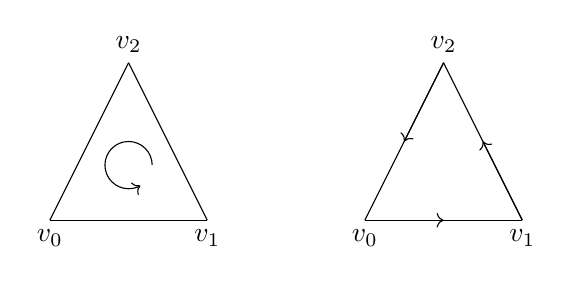
\begin{tikzpicture}
			\draw[] (4,0) node[below]{$v_0$}--(6,0)node[below]{$v_1$};
			\draw[] (6,0) -- (5,2) node[above]{$v_2$};
			\draw[] (5,2)--(4,0);
			%\draw (5,-1) node{$(v_0,v_1,v_2)$};	
			\draw[->] (5.3,0.7)arc[start angle=0, end angle=300,radius=0.3cm];
			%
			\draw[] (8,0) node[below]{$v_0$}--(10,0)node[below]{$v_1$};
			\draw[] (10,0) -- (9,2) node[above]{$v_2$};
			\draw[] (9,2)--(8,0);
			\draw[->](8,0)--(9,0);
			\draw[->](10,0)--(9.5,1);
			\draw[->](9,2)--(8.5,1);
		\end{tikzpicture}
	}
	\item 
	\parbox[c]{.5\linewidth}{\begin{align*}\partial_3(v_0,v_1,v_2,v_3)&=(v_1,v_2,v_3)-(v_0,v_2,v_3)\\
	&+(v_0,v_1,v_3)-(v_0,v_1,v_2)
	\end{align*}}%
\parbox[c]{.5\linewidth}{ 
	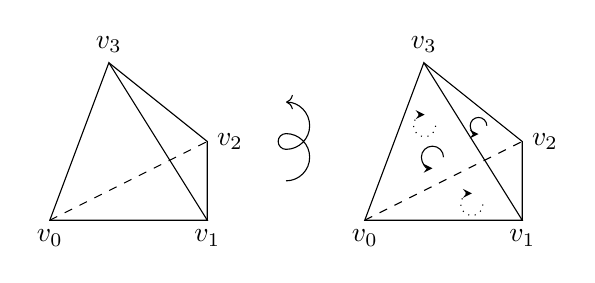
\begin{tikzpicture}
		\draw (0,0) node[below]{$v_0$}--(2,0)node[below]{$v_1$}--(0.75,2)node[above]{$v_3$}--cycle;
		\draw (2,0)--(2,1)node[right]{$v_2$}--(0.75,2);
		\draw[dashed] (0,0)--(2,1);
		\draw[->] (3,0.5) arc[start angle=-90, end angle=90, radius=0.3cm] arc [start angle=90, end angle=270,radius=0.1] arc[start angle=-90, end angle=90, radius=0.3];
		%
		\draw (4,0) node[below]{$v_0$}--(6,0)node[below]{$v_1$}--(4.75,2)node[above]{$v_3$}--cycle;
		\draw (6,0)--(6,1)node[right]{$v_2$}--(4.75,2);
		\draw[dashed] (4,0)--(6,1);
		%
		\draw[->,>=stealth](5.55,1.2)arc[start angle=0,end angle=270,radius=3pt];
		\draw[->,>=stealth,dotted](4.9,1.2)arc[start angle=0,end angle=-270,radius=4pt];
		\draw[->,>=stealth](5,.8)arc[start angle=0,end angle=270,radius=4pt];
		\draw[->,>=stealth,dotted](5.5,.2)arc[start angle=0,end angle=-270,radius=4pt];
	\end{tikzpicture}
	}

	\end{enumerate}
	
\end{examples}

%We will now consider the following diagram. (For the sake of readability, we deleted the dimension subscripts from the boundary operator)
%\begin{center}
%\begin{tikzcd}
%	C_\bullet:&\cdots \arrow[r, "\partial"] & C_{p+1}\arrow[r,"\partial"]&C_p\arrow[r,"\partial"]&C_{p-1}\arrow[r,"\partial"]&\cdots \\
%\end{tikzcd}

%\end{center}

Recall the following definition of a chain complex as can be found in Ferrario's book \parencite[p. 65]{fe}
\begin{definition}
	A chain complex $(\mathcal{C}_\bullet,\partial^\prime)$ is a graded abelian group $\{\mathcal{C}_n\}$ together with an endomorphism $\partial^\prime=\{\partial^\prime_n\}$ of degree\footnote{A graded abelian group G is a succession $\{G_i\mid i\in \Z\}$. For graded abelian groups $G$ and $K$, a morphism $g: G\to K$ is said to have degree $d$ if $f(G_n)\subset K_{n+d}$} $-1$ such that $(\partial^\prime)^2=0$.
\end{definition}

\begin{lemma}
	$(C_\bullet,\partial)$ is a chain complex.
\end{lemma}

\begin{proof}
	We need to show that $\partial_{p-1}\circ\partial_p\equiv 0$. It is not hard to prove this, it just requires some bookkeeping:
	
	Let $\sigma=(v_0,\dots,v_p)$ be an arbitrary $p$-chain, then
	\begin{align*}
		\partial_{p-1}\circ\partial_p(\sigma)&=\partial_{p-1}\left(\sum_{i=0}^{p}(-1)^i(v_0,\dots,\hat{v}_i,\dots,v_p)\right)=\sum_{i=0}^{p}(-1)^i\partial_{p-1}(v_0,\dots,\hat{v}_i,\dots,v_p)\\
		&=\sum_{i=0}^{p}(-1)^i\sum_{\parbox{.8cm}{\centering\scriptsize
				$j=0$\\$j\neq i$}}^{p}(-1)^j(v_0,\dots,\hat{v}_j,\dots,\hat{v}_i,\dots,v_p)
	\end{align*}
	Each of these term shows up twice with different signs. Thus, everything cancels.

\end{proof}

A common question for chain complexes is exactness. As we will see later in this chapter, $(C_\bullet,\partial)$ will only be exact for very special cases. 

Before we define the simplicial homology groups, we will introduce one more definition:

\begin{definition}\mbox{}
	\begin{enumerate}
		\item The kernel of $\partial_p: C_p(K)\to C_{p-1}(K)$ is called the group of $p$-cycles and denoted by $Z_p(K)$.
		\item The immage of $\partial_{p+1}: C_{p+1}(K)\to C_{p}(K)$ is called the group of $p$-boundaries and is denoted $B_p(K)$.
	\end{enumerate}
	
\end{definition}
The previous lemma states that $B_p(K)\subset Z_p(K)$.

Let us remind ourselves of what we wanted to do in \autoref{motivation}. We wanted to consider those closed curves (\emph{cycles}) that were not the \emph{boundary} of some part of the surface. With this in mind, we can now state the definition of simplical homology groups

\begin{definition}
	We define \[
	H_p(K):=Z_p(K)/B_p(K)=\ker \partial_p/\im \partial_{p+1}
	\]
	and call it the \textbf{$\mathbf{p}$-th simplicial homology goup of $\mathbf{K}$}.
\end{definition}
%TODO Examples
\begin{examples}\mbox{}
	\begin{enumerate}
%Point

\item Let us begin with the easiest example one can think of. Let $K$ be the simplicial complex consisting of only one 0-simplex (i.e. one vertex $v$). Clearly the chain complex then obviously reads

\begin{center}
\begin{tikzcd}
	C_1(K)\arrow[r,"\partial"]\arrow[d,equals]&C_0(K)\arrow[d,equals]\arrow[r,"\partial"]&\arrow[d,equals]0\\
	0\arrow[r,"\partial"]&\Z\langle v\rangle\arrow[r,"\partial"]&0
\end{tikzcd}
\end{center}
Then the homology groups are \[
H_0(K)\isom\Z,\quad H_{n>1}(K)=0
\]
%Circle
%%sphere as exercise at the end of handout
%Torus
%Klein bottle


%		\item Lets start with a simple triangulation\footnote{A triangulation of a space $T$ is a simplicial complex $X$ whose geometric realization $|X|$ is homeomorphic to $T$.}
%		 of $\Sp^2$ like the hollow tetrahedron (depicted in \autoref{hollow-tetrahedron}) \[X=\langle v_0v_1v_2,v_0v_1v_3,v_0v_2v_3,v_1v_2v_3 \rangle. \]
%			 	
%		 	\begin{figure}\centering
%		 		\begin{tikzpicture}
%		 		\draw (4,0) node[below]{$v_0$}--(6,0)node[below]{$v_1$}--(4.75,2)node[above]{$v_3$}--cycle;
%		 		\draw (6,0)--(6,1)node[right]{$v_2$}--(4.75,2);
%		 		\draw[dashed] (4,0)--(6,1);
%		 			\draw[->,>=stealth](5.55,1.2)arc[start angle=0,end angle=270,radius=3pt];
%		 			\draw[->,>=stealth,dotted](4.9,1.2)arc[start angle=0,end angle=-270,radius=4pt];
%		 			\draw[->,>=stealth](5,.8)arc[start angle=0,end angle=270,radius=4pt];
%		 			\draw[->,>=stealth,dotted](5.5,.2)arc[start angle=0,end angle=-270,radius=4pt];
%		 		\end{tikzpicture}
%		 		\caption{geometric realization of the hollow tetrahedron.\label{hollow-tetrahedron}}
%		 	\end{figure}
%	 It consists of four faces ($f_1=v_0v_1v_2, f_2=v_0v_1v_3$, $f_3=v_0v_2v_3, f_4=v_1v_2v_3$), six edges ($e_1=v_0v_1, e_2=v_0v_2, e_3=v_0v_3,$ $ e_4=v_1v_2, $ $e_5=v_1v_3, $ $e_6=v_2v_3$) and four vertices ($v_0,v_1,v_2,v_3$). Therefore, we find the simplicial chain complex to be
%	 \begin{tikzcd}
%	 	\Z\langle f_1,f_2,f_3f_4\rangle\arrow[r,"\partial_2"]&\Z\langle e_1,e_2,e_3,e_4,e_5,e_6\rangle\arrow[r,"\partial_1"]&\Z\langle v_0,v_1,v_2,v_3\rangle\arrow[r,"\partial_0"]&0
%	 \end{tikzcd}
% 
% Computing the boundaries and writing the results in a more user friendly fashion gives
% 
% \parbox[c]{.6\linewidth}{
% \begin{align*}
% 	\partial f_1=v_1v_2-v_0v_2+v_0v_1=e_1-e_2+e_4\\
% 	\partial f_2=v_1v_3-v_0v_3+v_0v_1=e_1-e_3+e_5\\
% 	\partial f_3=v_2v_3-v_0v_3+v_0v_2=e_2-e_3+e_6\\
% 	\partial f_4=v_2v_3-v_1v_3+v_1v_2=e_4-e_5+e_6
% \end{align*}}%
%\parbox[c]{.4\linewidth}{
%	$\partial_2=\begin{matrix}
%		 	&\begin{matrix}f_1	&f_2	&f_3	&f_4\end{matrix}\\
%		\begin{matrix}
%		e_1	\\
%		e_2	\\
%		e_3	\\
%		e_4	\\
%		e_5	\\
%		e_6	
%		\end{matrix}&
%		\begin{bmatrix}
%		1		&1		&0		&0\\
%		-1		&0		&1		&0\\
%		0		&-1		&-1		&0\\
%		1		&0		&0		&1\\
%		0		&1		&0		&-1\\
%		0		&0		&1		&1
%		\end{bmatrix}
%	\end{matrix}$	
%}
%
%\parbox[c]{.5\linewidth}{
%\begin{align*}
%	\partial e_1&=v_1-v_0,&&\partial e_2=v_2-v_0,&&\partial e_3=v_3-v_0,\\
%	\partial e_4&=v_2-v_1,&&\partial e_5=v_3-v_1,&&\partial e_6=v_3-v_1
%\end{align*}}%
%\parbox[c]{.5\linewidth}{$
%\quad\begin{matrix}
%	&\begin{matrix}e_1&e_2&e_3&e_4&e_5&e_6	\end{matrix}\\
%	\begin{matrix}v_0\\v_1\\v_2\\v_3\end{matrix}&
%	\begin{bmatrix}
%	-1	&-1	&-1	&0	&0	&0\\
%	1	&0	&0	&-1	&-1	&0\\
%	0	&1	&0	&1	&0	&-1\\
%	0	&0	&1	&0	&1	&1
%	\end{bmatrix}
%\end{matrix}$
%}
%We then find
%\begin{align*}
%\ker \partial_2&=\Z\langle f_1-f_2+f_3-f_4\rangle\\
%\ker \partial_1&=\Z\langle e_1-e_2+e_4,e_1-e_3+e_5, e_2-e_3+e_6 \rangle
%\end{align*}
%Then we have
%\begin{align*}
%	H_2(\Sp^2)&=\ker \partial_2/\im \partial_3=\ker \partial_2=\Z\langle f_1-f_2+f_3-f_4\rangle\simeq\Z\\
%	H_1(\Sp^2)&=\ker \partial_1/\im \partial_2\simeq\Z^3/\Z^3\simeq 0\\
%	H_0(\Sp^2)&=\ker\partial_0/\im \partial_1\simeq \Z^4/\Z^3\simeq \Z\\
%	H_n(\Sp^2)&=0\quad \text{for $n>2$}
%\end{align*}
%

%\item The Torus (see \autoref{torus}) is a little more difficult. Unfortunately, the simplest (simplicial) triangulation is depicted in \autoref{triangulation-torus}. This triangulation would lead to boundary operators in the form of  $27\times 18$  and  $8\times 27$ matrices respectively.  The resulting homology groups are:
%\[
%H_0=\Z,\quad H_1=\Z^2,\quad H_2=\Z,\quad H_{n>2}=0
%\]
%Even tough these aren't hard to compute, it is very tedious and therefore wont be presented here.\footnote{By introducing the concept of cellular homology, this can be simplified to $3\times 2$ and $1\times 3$ matrices via the \glqq(non-simplicial)  triangulation\grqq:	
%	
%\begin{tikzpicture}[scale=0.5]
%	\draw[->] (-5,0) node[below]{$v_0$}--(-4,0) node[below]{b};
%	\draw[->] (-5,2) node[above]{$v_0$}--(-4,2) node[above]{b};
%	\draw[->] (-5,0)--(-5,1) node[left]{a};
%	\draw[->] (-3,0) node[below]{$v_0$}--(-3,1) node[right]{a};
%	\draw[->] (-5,0)--(-4,1) node[above]{$c$};
%	\draw[->] (-4,1)--(-3,2);
%	\draw (-5,0)--(-3,0)--(-3,2) node[above]{$v_0$}--(-5,2)--cycle;
%\end{tikzpicture}
%
%	 Cellular and simplicial homology actually coincide. However we currently lack the framework for cellular homology}
%
%\begin{figure}
%	
%\parbox[c]{.5\linewidth}{\centering
%\begin{tikzpicture}
%	\draw[->] (-5,0) node[below]{$v_0$}--(-4,0) node[below]{b};
%	\draw[->] (-5,2) node[above]{$v_0$}--(-4,2) node[above]{b};
%	\draw[->] (-5,0)--(-5,1) node[left]{a};
%	\draw[->] (-3,0) node[below]{$v_0$}--(-3,1) node[right]{a};
%	\draw (-5,0)--(-3,0)--(-3,2) node[above]{$v_0$}--(-5,2)--cycle;
%\end{tikzpicture}}%
%\parbox[c]{.5\linewidth}{\centering
%\begin{tikzpicture}
%	\draw (0,0)--(6,0)--(6,6)--(0,6)--cycle;
%	\draw (2,0)--(2,6);
%	\draw (4,0)--(4,6);
%	\draw (0,2)--(6,2);
%	\draw (0,4)--(6,4);
%	\draw (0,4)--(2,6);
%	\draw (0,2)--(4,6);
%	\draw (0,0)--(6,6);
%	\draw (2,0)--(6,4);
%	\draw (4,0)--(6,2);
%\end{tikzpicture}	
%}
%\parbox[t]{.5\linewidth}{\captionsetup{width=.9\linewidth}
%\caption{The fundamental polygon of the torus.\label{torus}}}%
%\parbox[t]{.5\linewidth}{\captionsetup{width=.9\linewidth}\caption{A simplicial triangulation of the torus.\label{triangulation-torus}}}
%\end{figure}
%
%We see that the homology groups for the Sphere and the Torus do not agree in every dimension. Since homotopy equivalent spaces 
%have isomorphic homology groups (we will show that later), we find that the sphere cannot be homotopy equivalent to the torus.

\item We will now consider the circle. This can be triangulated as an empty triangle, i.e.
\begin{center}
	
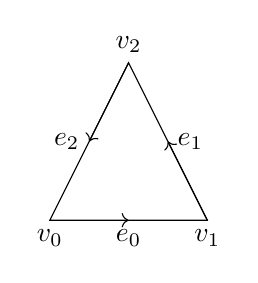
\begin{tikzpicture}
	\draw[->] (0,0)--(1,0) node[below]{$e_0$};
	\draw[->] (2,0)--(1.5,1)node[right]{$e_1$};
	\draw[->] (1,2)--(0.5,1)node[left]{$e_2$};
	\draw (0,0) node[below]{$v_0$}--(2,0) node[below]{$v_1$}--(1,2) node[above]{$v_2$}--cycle;
\end{tikzpicture}
\end{center}

We easily find 
\[
\partial_1=\begin{bmatrix}
-1&0&1\\1&-1&0\\0&1&-1
\end{bmatrix},\quad \partial_0\equiv 0
\]
Therefore,
\[H_1(\Sp^1)\isom\Z/0\isom\Z,\quad H_0(\Sp)\isom\Z^3/\Z^2\isom\Z
\]
%\item 
%Now that we have considered the circle, we might also be interested in the $2$-ball $B^2$. The triangulation is very easy this time. It is just one 2-dimensional simplex:
%\begin{center}
%\begin{tikzpicture}
%\draw[] (4,0) node[below]{$v_0$}--(6,0)node[below]{$v_1$};
%\draw[] (6,0) -- (5,2) node[above]{$v_2$};
%\draw[] (5,2)--(4,0);
%%\draw (5,-1) node{$(v_0,v_1,v_2)$};	
%\draw[->] (5.3,0.7)arc[start angle=0, end angle=300,radius=0.3cm];
%\end{tikzpicture}
%
%We find that $\partial_1$ and $\partial_0$ are the same as before and $\partial_2$ can be expressed as
%\[
%\partial_2=\begin{bmatrix}
%1\\1\\1
%\end{bmatrix}
%\]
%We then find
%\[
%H_2(B^2)=0,\quad H_1(B^2)=0,\quad H_0(B^2)=\Z
%\]
%
%\end{center}
	\end{enumerate}
%For the torus\parencite[p. 180f.]{ar}:

Let $K$ be a triangulation of the torus. If we orient all the 2-simplices of $K$ compatibly, take this sum, and compute the boundary of this sum, then  each edge of the triangulation occurs exactly twice in the result, once with each of its two possible orientations. So we have a two-dimensional cycle. It is elementary to check that any other 2-cycle has to be an integer multiple of this one. (For suppose the oriented triangle $(a,b,c)$ occurs in a 2-cycle with coefficient $\lambda$, then $\lambda(b,c)$ automatically appears in its boundary. Now the edge spanned by $b$ and $c$ lies in precisely one other triangle of $K$ whose third vertex we denote by $d$. The only way we can rid ourselves of the above term $\lambda(b,c)$ is to orient this adjacent triangle as $(d,c,b)$ in other words, compatibly with $(a,b,c)$, and include it in our cycle with the same coefficient $\lambda$. Going round the complex in this way, we see we must orient all simplexes compatibly, and give them all the same coefficient.) Since there are no 3-simplices in a triangulation of the torus, there are no bounding cycles, and therefore $H_2(K)$ is isomorphic to $\Z$.

%Just about punctuerd Torus
%If we now change to a triangulation of the punctured torus, there are no 2-cycles, since even if we include all the triangles oriented compatibly as above, when we compute the boundary we are left with those edges which form the boundary of the hole in the torus. So the second homology group is zero.

for the klein bottle:
The second homology group of a triangulation of the Klein bottle is zero. There are no 2-cycles because it is not possible to orient all the 2-simplices of a triangulation compatibly, since the Klein bottle is nonorientable.

Therefore the homology groups for the torus and the Klein bottle are not isomorphic in every dimension. Thus, they can't be homeomorphic.

We will consider the (more interesting) cases of the torus and the Klein Bottle shortly. But we need a preliminary result first because even though the same method as before can be applied in theory, this is not very practical since the matrices would uncomfortably large.

\begin{lemma}%Lemma 6.1 Munkres
	Let $L$ be the complex depicted in figure \ref{rectangle-tri}, whose underlying space is a rectangle. Let $\mathrm{Bd} L$ denote the complex whose space is the boundary of the rectangle. Orient each 2-simplex $\sigma_i$ of $L$ counterclockwise. Orient the 1-simplices arbitrarily. Then:
	\begin{enumerate}
		\item Every 1-cycle of $L$ is homologous to a 1-cycle carried by $\mathrm{Bd} L$.
		\item If $d$ is a 2-chain of $L$ and if $\partial d$ is carried by $\mathrm{Bd}L$, then $d$ is a multiple of the chain $\sum \sigma_i$.
	\end{enumerate} 
\end{lemma}
% A chain c is carried by a subcomplex $L$ of $K$ if $c$ has value 0 on every simplex that is not in $L$. We say two chais are homologous if they only differ by a boundary.


\begin{figure}\begin{center}
	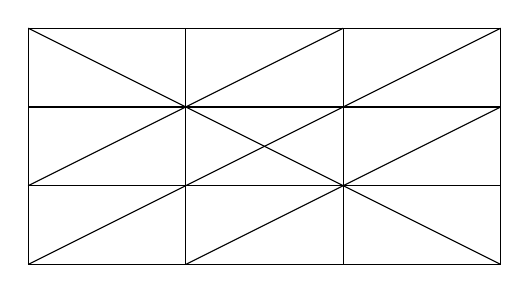
\begin{tikzpicture}[yscale=0.5]
	\draw (0,0)--(6,0)--(6,6)--(0,6)--cycle;
	\draw (2,0)--(2,6);
	\draw (4,0)--(4,6);
	\draw (0,2)--(6,2);
	\draw (0,4)--(6,4);
	\draw (0,6)--(6,0);
	\draw (0,2)--(4,6);
	\draw (0,0)--(6,6);
	\draw (2,0)--(6,4);
	\end{tikzpicture}	
	\caption{Complex whose underlying space is a rectangle.\label{rectangle-tri}}

\end{center}
\end{figure}


\begin{proof}
	We will prove the second statement fist. If $\sigma_i$ and $\sigma_j$ have an edge $e$ in common, then $\partial d$ must have value 0 on $e$. It follows that $d$ must have the same value $\sigma_i$ as it does in $\sigma_j$. Continuing this process, we see that $d$ has the same value on every oriented 2-simplex $\sigma_i$.
	
	For the second part, let $c$ be be a 1-chain of $L$. We will \glqq push it off \grqq{} the 1-simplices in the following way:
	
	We concentrate on the center at first. There we notice the structure as depicted in figure \ref{zoom-in}.
	
	\begin{figure}
		\begin{center}
			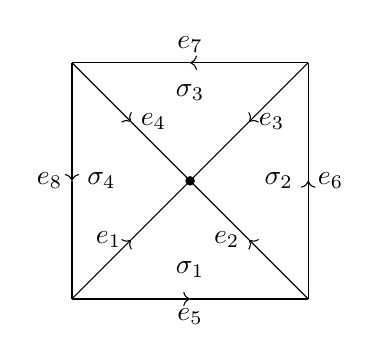
\begin{tikzpicture}[scale=1.5]
				\draw[->] (0,0)->(1,0) node[below]{$e_5$};
				\draw (1,0)--(2,0);
				\draw[->] (2,0)->(2,1) node[right]{$e_6$};
				\draw (2,1)--(2,2);
				\draw[->] (2,2)->(1,2) node[above]{$e_7$};
				\draw (1,2)--(0,2);
				\draw[->] (0,2)->(0,1) node[left]{$e_8$};
				\draw (0,1)--(0,0);
				\draw[->] (0,0)--(0.5,0.5) node[left]{$e_1$};
				\draw (0.5,0.5)--(1.5,1.5);
				\draw (1.5,0.5)--(0.5,1.5);
				\draw[->](2,2)--(1.5,1.5) node[right]{$e_3$};
				\draw[->](2,0)--(1.5,0.5) node[left]{$e_2$};
				\draw[->](0,2)--(0.5,1.5) node[right]{$e_4$};
				\filldraw (1,1) circle (1pt);
				\draw (1,0.25) node{$\sigma_1$};
				\draw (1,1.75) node{$\sigma_3$};
				\draw (0.25,1) node{$\sigma_4$};
				\draw (1.75,1) node{$\sigma_2$};
			\end{tikzpicture}
			\caption{Structure of center. 2-simplices are oriented counterclockwise\label{zoom-in}}
		\end{center}
	\end{figure}

Let $c$ denote a 1-chain with value $a$ on $e_1$. Then $c$ is clearly homologous to the chain $c_1=c+\partial(a\sigma_1)$. The resulting 1-chain $c_1$ vanishes on $e_1$. We have \glqq pushed it off\grqq{} $e_1$. We can apply this multiple times for other edges until we arrive at a chain $c_2$ which is carried by the subcomplex depicted in figure \ref{skelleton}
\begin{figure}
	\begin{center}
		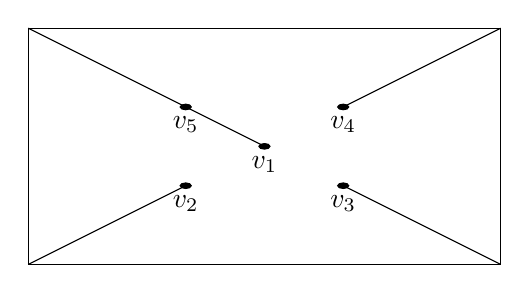
\begin{tikzpicture}[yscale=0.5]
		\draw (0,0)--(6,0)--(6,6)--(0,6)--cycle;
		\draw (0,6)--(3,3);
		\draw (0,0)--(2,2);
		\draw (6,0)--(4,2);
		\draw (6,6)--(4,4);
		\filldraw (2,2)circle(2pt) node[below]{$v_2$};
		\filldraw (3,3)circle(2pt) node[below]{$v_1$};
		\filldraw (2,4)circle(2pt) node[below]{$v_5$};
		\filldraw (4,4)circle(2pt) node[below]{$v_4$};
		\filldraw (4,2)circle(2pt) node[below]{$v_3$};
		\end{tikzpicture}
		\caption{Subcomplex that carries $c_2$.\label{skelleton}}	
	\end{center}
\end{figure} 

Since our original $c$ is a cycle, $c_2$ must be carried by $\mathrm{Bd} L$, because otherwise $\partial c_2$ 
%TODO Check boundary here? In Munkres no boundary.
would have non-zero coefficients on one or more of the vertices $v_1, \dots,v_5$.
\end{proof}

\begin{theorem}
	Let $T$ denote the complex represented by the labeled rectangle $L$ of Figure \ref{torus-tri}. Its underlying space is the torus. Then:
	\[H_1(T)\isom \Z\oplus\Z \qandq H_2(T)\isom \Z.\]
	Orient each 2-simplex of $L$ counterclockwise; use the induced orientation of the 2-simplices of T; Let $\gamma$ denote their sum. Let 
	\begin{align*}
	w_1=&[a,b]+[b,c]+[c,a],\\
	z_1=&[a,d]+[d,e]+[e,a].
	\end{align*}
	Then $\gamma$ generates $H_2(T)$ and $w_1$ and $z_1$ represent a basis for $H_1(T)$.
\end{theorem}

\begin{figure}\begin{center}
		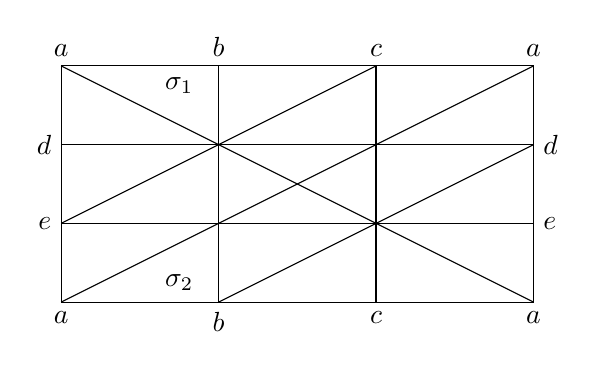
\begin{tikzpicture}[yscale=0.5]
		\draw (0,0) node[below]{$a$}--(6,0)node[below]{$a$}--(6,6)node[above]{$a$}--(0,6)node[above]{$a$}--cycle;
		\draw (2,0)node[below]{$b$}--(2,6)node[above]{$b$};
		\draw (4,0)node[below]{$c$}--(4,6)node[above]{$c$};
		\draw (0,2)node[left]{$e$}--(6,2)node[right]{$e$};
		\draw (0,4)node[left]{$d$}--(6,4)node[right]{$d$};
		\draw (0,6)--(6,0);
		\draw (0,2)--(4,6);
		\draw (0,0)--(6,6);
		\draw (2,0)--(6,4);
		\draw (1.5,5.5)node{$\sigma_1$};
		\draw (1.5,0.5) node{$\sigma_2$};
		\end{tikzpicture}	
		\caption{Labeled Complex whose underlying space is a torus.\label{torus-tri}}
		
	\end{center}
\end{figure}
\begin{proof}
	Let $g: |L|\to |T|$ be the pasting (gluing) map; let $A=g(|\mathrm{Bd} L)$. Then $A$ is homeomorphic to\footnote{The wedge sum is the disjoint union where two points are identified.} $\Sp^1\wedge \Sp^1$ as depicted in figure \ref{wege-of-s1}. Orient the 1-simplices of $T$ arbitrarily. Since $g$ only identifies simplices in $\mathrm{Bd} L$, we find the same statements as above with identical arguments.
	\begin{enumerate}
		\item \label{gen-1}Every 1-cycle of $T$ is homologous to a 1-cycle carried by $A$.
		\item \label{gen-2}If $d$ is a 2-chain of $T$ and if $\partial d$ is carried by $A$, then $d$ is a multiple of $\gamma$.
	\end{enumerate}
	Additionally, we find here
	\begin{enumerate}\setcounter{enumi}{2}
		\item \label{torus-1} If $c$ is a 1-cycle of $T$ carried by $A$, then $c$ is of the form $nw_1+mz_1$.
		\item \label{torus-2}$\partial \gamma=0$.
	\end{enumerate} 
	\begin{figure}
		\begin{center}
			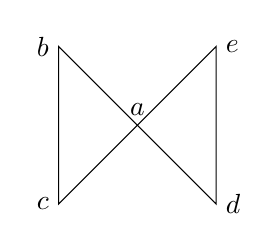
\begin{tikzpicture}
				\draw (-1,-1) node[left]{$c$}--(0,0) node[above]{$a$}--(-1,1) node[left]{$b$}--cycle;
				\draw (0,0)--(1,-1) node[right]{$d$}--(1,1)node[right]{$e$}--cycle;
			\end{tikzpicture}
			\caption{$A$ is homeomorphic to $\Sp^1\wedge \Sp^1$\label{wege-of-s1}}
		\end{center}
	\end{figure}

The statement in item \ref{torus-1} is clear by looking at figure \ref{wege-of-s1}. For item \ref{torus} we need to see the following: 
It is clear that $\partial\gamma$ vanishes on any 1-simplex not contained in $A$. By direct computation one can see that $\partial\gamma$ also vanishes on all 1-simplices in $A$. The 1-simplex $[a,b]$ appears as a face of $\sigma_1$ and $\sigma_2$ and no other simplices. If we evaluate $\partial\sigma_1$ the elementary chain $[a,b]$ is assigned the value $-1$ and evaluating $\partial\sigma_2$ gives $+1$ for $[a,b]$.

Combining all of the results above yields the homology groups of $T$:
Every 1-cycle of $T$ is homologous to a 1-cycle of the form $c=nw_1+mz_1$ by \ref{gen-1} and \ref{torus-1}. Such a cycle bounds only if it is trivial: If $c=\partial d$ for some $d$, then by virtue of \ref{gen-2} $d=p\gamma$ for some integer $p$. By \ref{torus-2} we know that $\partial\gamma=0$, so $c=0$. Therefore,
\[H_1(T)\isom\Z\oplus\Z; \]
with base elements $w_1$ and $z_1$.

For dimension 2,we find that any 2-cycle $d$ of $T$ must be of the form $p\gamma$ for some $p$ by virtue of \ref{gen-2}. Such a 2-chain is always a cycle, by \ref{torus-2}, and there are no 3-chains whose boundary they could be, hence
\[
H_2(T)\isom \Z
\]
with generator $\gamma$.
\end{proof}




\begin{theorem}
	let $S$ denote the complex represented by the labeled rectangle of figure \ref{klein-tri}; its underlying space is the Klein bottle. Then 
	\[H_1(S)\isom\Z\oplus\Z_2\qandq H_2(S)=0.\]
	The torsion element of $H_1(S)$ is represented by the chain $z_1$, and a generator for the group $H_1(S)$ modulo torsion is represented by $w_1$, where
	\begin{align*}
		w_1&=[a,b]+[b,c]+[c,a]\\
		z_1&=[a,d]+[d,e]+[e,a].
	\end{align*}
\end{theorem}
\begin{figure}\begin{center}
		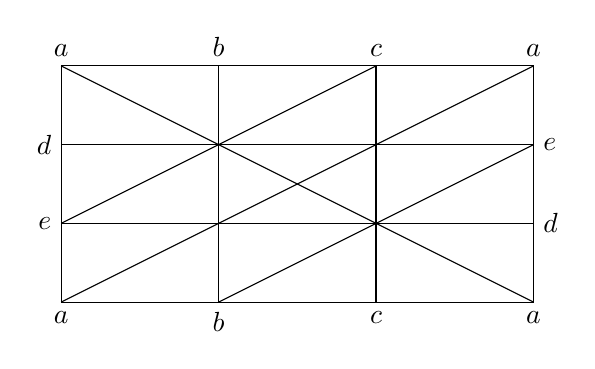
\begin{tikzpicture}[yscale=0.5]
		\draw (0,0) node[below]{$a$}--(6,0)node[below]{$a$}--(6,6)node[above]{$a$}--(0,6)node[above]{$a$}--cycle;
		\draw (2,0)node[below]{$b$}--(2,6)node[above]{$b$};
		\draw (4,0)node[below]{$c$}--(4,6)node[above]{$c$};
		\draw (0,2)node[left]{$e$}--(6,2)node[right]{$d$};
		\draw (0,4)node[left]{$d$}--(6,4)node[right]{$e$};
		\draw (0,6)--(6,0);
		\draw (0,2)--(4,6);
		\draw (0,0)--(6,6);
		\draw (2,0)--(6,4);
		\end{tikzpicture}	
		\caption{Labeled Complex whose underlying space is the Klein bottle.\label{klein-tri}}
		
	\end{center}
\end{figure}
\begin{proof}
	Let $g$ and $A$ be as before with the obvious changes. Again, $A$ is homeomorphic to $\Sp^1\wedge \Sp^1$. Orient all 2-simplices of $S$ as before and let $\gamma$ be their sum. Orient the 1-simplices arbitrarily. Once more, Statements \ref{gen-1} and \ref{gen-2} from the previous proof hold for the same reason as before. Since $A$ is the wedge sum of two circles again, \ref{torus-1} holds again. However, condition \ref{torus-2} needs to be modified:
	\begin{enumerate}
		\setcounter{enumi}{3}
		\item $\partial \gamma=2z_1$\label{klein-2}.
	\end{enumerate}
	This result can be obtained via a direct calculation similar from what we did before.
	
	By \ref{gen-1} and \ref{torus-1} we know that every 1-cycle of $S$ is homologous to a cycle of the form $c=nw_1+mz_1$. If $c$ is a boundary for some $d$, then \ref{gen-2} implies $d=p\gamma$. Thus, $\partial d=2pz_1$. Therefore $nw_1+mz_1$ bounds if and only if $m$ is even and $n$ is zero. Thus,
	\[H_1(S)\isom\Z\oplus\Z_2\]
	The cycle $z_1$ represents the torsion element, and $w_1$ represents a generator of the infinite cyclic group $H_1(S)/T_1(S)$.
	
	For the second homology group, note that any 2-cycle $d$ of $S$ must be of the form $p\gamma$ by \ref{gen-2}. \ref{klein-2} implies that $p\gamma$ is not a cycle, hence
	\[
	H_2(S)=0.
	\]
\end{proof}
\end{examples}


\section{\SH{} Groups with $\mathbb{Z}/2\mathbb{Z}$ Coefficients}

Let us remind ourselves of the definition for $p$-chains (Definition \ref{def-chain}):
\begin{quotation}
	Let $K$ be a simlicial complex. A \textbf{$p$-chain} on $K$ is a function $c$ from the set of oriented $p$-simplices of $K$ to the integers such that:
	\begin{enumerate}
		\item $c(\sigma)=-c(\sigma^\prime)$ if $\sigma$ and $\sigma^\prime$ are opposite orientations of the same simplex.
		\item $c(\sigma)=0$ for all but finitely many oriented $p$-simplices $\sigma$.
	\end{enumerate}
\end{quotation}

There is actually no reason (other than our familiarity with it) to restrict ourselves to the integers here. In fact, the same statements hold true for any abelian group $G$ and it can be helpful to consider other groups than the integers. To denote the change of our underlying group, we use the notation
\[
C_n(K;G)\qandq H_n(K;G)
\]
for the group of chains and the homology group of $K$ with coefficients in $G$.

Since the group of chains with integer coefficients $C_n(K;\Z)=C_n(K)$ merely consists of linear combinations of elementary chains with integer coefficients, there is a neat way to derive $C_n(K;G)$ if $C_n(K;\Z)$ is already known. We find that
\[
C_n(K;G)\simeq C_n(K;\Z)\otimes_\Z G,
\]
which leads to many interesting phenomena. The same holds for homology groups if the coefficient ring is a field of characteristic zero.
%TODO No it doesn't. Need Universal coefficient theorem, but over a field Ext is zero so it holds for fields.



%This might be a good time to remember the fundamental theorem of finitely generated abelian groups (such as the homology groups) as it can be found in Munkres' book \cite[see ][Theorem 4.3, p. 24]{mu}:
%\begin{theorem}[The fundamental theorem of finitely generated abelian groups]
%	Let $G$ be a finitely generated abelian group. Let $T$ be its torsion subgroup.Then there exists a free abelian subgroup $H$ of $G$ having finite rank such that $G=H\oplus T$. 
%\end{theorem}
%
%Since there is no possibility of torsion after taking the tensor product with a field of characteristic 0, we find that for any such field $\mathbb{K}$ the homology group with coefficients in $\mathbb{K}$ is a $\mathbb{K}$-vectorspace.


A special case is the coefficient ring $\Z/2\Z$, since here $-1=1$. Hence, we no longer have to worry about orientation. Therefore, this ring is often used if the considered manifolds might or might not be orientable.

%TODO Examples: RP^2, klein bottle

\begin{examples}
	We shall review the examples from the previous chapter, namely the Torus and the Klein bottle. With the same argument we see that
	\begin{align*}
		H_1(T;\Z_2)\isom& \Z_2\otimes\Z_2\\
		H_2(T;\Z_2)\isom& \Z_2.
	\end{align*}
	
	For the Klein bottle $S$, the argument needs to be changed slightly. With $\Z_2$ coefficients, the basic 2-chain $\gamma$, which is the sum of the 2-simplices of $S$, has boundary zero. This leads to the conclusion that 
	\begin{align*}
		H_1(S;\Z_2)&\isom \Z_2\oplus \Z_2\\
		H_2(S;\Z_2)&\isom \Z_2
	\end{align*}

	More generally, one can show that Homology with $\Z_2$ coefficients does not distinguish between orientable and non-orientable surfaces of genus $g$.
\end{examples}


\section{Functoriality Property}
We will now explore how homotopy behaves under continuous functions. We will begin with the following definition and lemma from Munkres' book \cite[lemma 12.1, p. 62]{mu}:

\begin{definition}
	Let $f: K\to L$ be a simplicial map. If $v_0\dots v_p$ is a simplex of $K$, then the points $f(v_0)\dots f(v_p)$ span a simplex of $L$. we define a homomorphism $f_\sharp: C_p(K)\to C_p(L)$ by defining it on oriented simplices as follows:
	\[
	f_\sharp([v_0,\dots,v_p])=\begin{cases}
	[f(v_0),\dots, f(v_p)],& \text{if } f(v_0),\dots, f(v_p) \text{ are distinct}\\
	0,&\text{otherwise}
	\end{cases}
	\]
	
	The family $\{f_\sharp\}$ is called the chain map induced by the simplicial map $f$.
\end{definition}

This gives rise to the following diagram:

\begin{center}
	
\begin{tikzcd}
	\cdots\arrow[r,"\partial"]&C_p(K)\arrow[r,"\partial"]\arrow[d,"f_\sharp"]&C_{p-1}(K)\arrow[r,"\partial"]\arrow[d,"f_\sharp"]&C_{p-2}(K)\arrow[r,"\partial"]\arrow[d,"f_\sharp"]&\cdots
	\\
	\cdots\arrow[r,"\partial"]&C_p(L)\arrow[r,"\partial"]&C_{p-1}(L)\arrow[r,"\partial"]&C_{p-2}(L)\arrow[r,"\partial"]&\cdots
\end{tikzcd}
\end{center}

This of course raises the question whether this diagram commutes or not. 
\begin{lemma}
	The homomorphism $f_\sharp$ commutes with $\partial$; therefore $f_\sharp$ induces a homomorphism $f_\ast:H_p(K)\to H_p(L)$
\end{lemma}

\begin{proof}

	Let $\tau$ denote the simplex of $L$ that is spanned by $f(v_0),\dots,f(v_p)$. We need to check 
	\begin{equation}\label{comm}
		\partial f_\sharp([v_0,\dots,v_p])=f_\sharp(\partial[v_0,\dots,v_p])
	\end{equation}
	\begin{description}
		\item[Case 1 $\dim\tau=p$:] Clearly, this requires $f(v_0),\dots,f(v_p)$ to be distinct. Therefore the statement follows directly from the definitions. %TODO check closely
		\item[Case 2 $\dim\tau\leq p-2$:] Here, the left side of \eqref{comm} vanishes because $f(v_0),\dots,f(v_p)$ are not distinct. The right side also vanishes, since for every $i$, at least two of the points $f(v_0),\dots,\hat{f}(v_i),\dots,f(v_p)$ are the same.%TODO this is too close to the source-> reformulate
		\item[Case 3 $\dim\tau=p-1$:] We will assume the following ordering of vertices:
		\begin{equation}\label{cond}
		f(v_0)=f(v_1), \qqandqq f(v_1),\dots,f(v_p) \text{ are distinct.}
		\end{equation}
		Similarly, to the previous case, the left side of \eqref{comm} vanishes and the right side reads
		\[
		[f(v_1)f(v_2),\dots,f(v_p)]-[f(v_0),f(v_2),...,f(v_p)].
		\]
		By \eqref{cond} this also vanishes. 
	\end{description}

To show the second part of the lemma, we need to understand how $f_\sharp$ acts on boundaries and cycles. Let $c$ be an arbitrary cycle of $K$, i.e. $\partial c=0$. Then by \eqref{comm}, we find $\partial f_\sharp (c)=f_\sharp (\partial c)=f_\sharp(0)=0$.

Now, let $b$ be an arbitrary boundary, i.e. there exists some $d$ with $b=\partial d$. Then, $f_\sharp(b)=f_\sharp(\partial d)=\partial f_\sharp(d)$. 

We have thereby shown that $f_\sharp$ maps boundaries (cycles) of $K$ to boundaries (cycles) of $L$. 
\end{proof}

With this in mind we can now state the functional properties of these homomorphisms. We do this by following Munkres' book \cite[Theorem 12.2, p. 53]{mu} once more.

\begin{theorem}[functorial properties I]\label{func-prop1}\mbox{}
	\begin{enumerate}
		\item Let $id: K\to K$ be the identity simplicial map. Then $id_\ast: H_p(K)\to H_p(K)$ is the identity homomorphism.
		\item Let $f:K\to L$ and $g: L\to M$ be simplicial maps. Then $(g\circ f)_\ast=g_\ast\circ f_\ast$; That is, the following diagram commutes:
		
		\begin{center}
			
		\begin{tikzcd}
			H_p(K)\arrow[rd,"f_\ast"]\arrow[rr,"(g\circ f)_\ast"]
			&&H_p(M)\\
			&H_p(L)\arrow[ru,"g_\ast"]&
		\end{tikzcd}
	\end{center}
	\end{enumerate}
\end{theorem}



\begin{proof}
	The first part of the Theorem is pretty obvious. The second part follows immediately form $(g_\sharp\circ f_\sharp)=(g\circ f)_\sharp$. To see this, we shall consider vertices $v_0,\dots,v_p$ that span a simplex in $K$.
	Then by definition 
	\[
	f_\sharp([v_0,\dots,v_p])=\begin{cases}
	[f(v_0),\dots,f(v_p)],& \text{if }f(v_0),\dots,f(v_p) \text{ are distinct},\\
	0,& \text{otherwise}
	\end{cases}
	\]
	Thus,
	\begin{align*}
	g_\sharp\circ f_\sharp([v_0,\dots,v_p])=&\begin{cases}
	[g\circ f(v_0),\dots,g\circ f(v_p)],& \text{if }g\circ f(v_0),\dots,g\circ f(v_p) \text{ are distinct},\\
	0,& \text{if }g\circ f(v_0),\dots,g\circ f(v_p) \text{ aren't distinct}\\
	0,& \text{if }f_\sharp([v_0,\dots,v_p])=0
	\end{cases}\\
	=&\begin{cases}
	[g\circ f(v_0),\dots,g\circ f(v_p)],& \text{if }g\circ f(v_0),\dots,g\circ f(v_p) \text{ are distinct},\\
		0,& \text{otherwise}
	\end{cases}\\
	&=(g\circ f)_\sharp([v_0,\dots,v_p])
	\end{align*}
\end{proof}


\begin{corollary}\label{baby-case}
	Let $f: K\to L$ be a bijective simplicial map such that its inverse is also a simplicial map. Then \[
	\forall p\geq 0:\quad H_p(K)\isom H_p(L)
	\]\qed
\end{corollary}

This already gives the main Idea for the next section.
%TODO old frontier

Let us remind ourselves of the general simplicial approximation theorem, as it can be found in Munkres' book \cite[Thm. 16.5, p. 85]{mu}:

\begin{theorem}[The general simplicial approximation theorem]
	Let $K$ and $L$ be complexes; let $h: |K|\to |L|$ be a continuous map. There exists a subdivision $K^\prime$ of $K$ such that $h$ has a simplicial approximation $f:K^\prime \to L$.
\end{theorem}

We will further need the following definition again for Munkres' book \cite[p. 100]{mu}:
\begin{definition}
	Let $K$ and $L$ be simplicial complexes; let $h:|K|\to |L|$ be a continuous map. Choose a subdivision $K^\prime$ of $K$ such that $h$ has a simplicial approximation $f:K^\prime\to L$ (such exists by virtue of the previous theorem). Let $\lambda:C_\bullet(K)\to C_\bullet(K^\prime)$ be the subdivision operator. We define the homomorphism induced by $h$ 
	\[
	h_\ast: H_p(K)\to H_p(L)
	\]
	via
	\[
	h_\ast=f_\ast\circ \lambda_\ast.
	\]
\end{definition}

%TODO well definedness

Since this definition involves several choices, we need to make sure, that the resulting homomorphism isn't dependent on these choices. We do this in two steps. Firstly, notice that for some choice of a subdivision $K^\prime$ two simplicial approximations, then these are contiguous and therefore induce the same homomorphism $f_\ast\equiv g_\ast$ (see Theorems \ref{chain_hom->invariant} and \ref{contiguous->chain_hom}).

Let $\iota: K^\prime\to K $ be a simplicial approximation to the identity map of $K$, then $\lambda_\ast=(g_\ast)^{-1}$, hence
\[
h_\ast=f_\ast\circ(g_\ast)^{-1}
\]

Secondly, we will now use this to show that $h_\ast$ doesn't depend on the choice of subdivision $K^\prime$ either. Let $K^\pprime$ be another subdivision of $K$ such that $h$ has a simplicial approximation mapping $K^\pprime$ to $L$. We will see that the induced homomorphism $h_\ast$ does not change if we use substitute $K$ with $K^\pprime$ in its definition.

We will first explore the special case that $|K|$ has a simplicial approximation $k: K^\pprime\to K^\prime$

\begin{center}
	
\begin{tikzcd}
	&&K\\
	K^\pprime\arrow[r,"k"]&K^\prime\arrow[ru,"g"]\arrow[rd,"f"]\\
	&&L	
\end{tikzcd}
\end{center}

Let $h_\ast^\prime$ be the induced homomorphism defined via $K^\pprime$. We can then write
\[
h_\ast^\prime(f\circ k)_\ast\circ(g\circ k)_\ast^{-1}=(f_\ast\circ k_\ast)\circ(g_\ast\circ k_\ast)^{-1}=f\circ g_\ast^{-1}=g_\ast\circ\lambda_\ast=h_\ast
\]

We generalize this method by considering a subdivision $K\ppprime$ of $K$ such that the identity map has simplicial approximations
\[
k_1: K^\ppprime\to K^\prime\qandq k_2: K^\ppprime\to K^\pprime.
\]

We can now use this subdivision to construct a homomorphism $h_\ast^\pprime$. By our previous work, we already know that 
\[
h_\ast^\prime=h_\ast^\pprime=h_\ast
\]

%TODO functorial properties
We are now able to generalize \autoref{func-prop1}
\begin{theorem}[functorial properties II]\label{func-prop2}
	The identity map $id: |K|\to |K|$ induces the identity homomorphism $i_\ast: H_p(K)\to H_p(K)$. If $h:|K|\to|L|$ and $k:|L|\to |M|$ are continuous maps, then $(k\circ h)_\ast=k_\ast\circ h_\ast$.
\end{theorem}
\begin{proof}
	The first part is elementary. For the second part, choose simplicial approximations as follows:
	
	\begin{tabular}{c|>{simplicial approximation to }l}
		$f_0: L^\prime\to M$&  $k$\\
		$g_0: L^\prime\to L$& the identity on $|L|$\\
		$f_1: K^\prime\to L^\prime$& $h$\\
		$g_1: K^\prime\to K$& the identity on $|K|$
	\end{tabular}

\begin{center}
	
	\begin{tikzcd}
		\left|K\right|\arrow[r,"h"]&\left|L\right|\arrow[r,"k"]&\left|M\right|\\
		K&L&M\\
		&L^\prime\arrow[u,"g_0"]\arrow[ur,"f_0"]\\
		K^\prime\arrow[uu,"g_1"]\arrow[ur,"f_1"]
	\end{tikzcd}
\end{center}
With these choices, $f_0\circ f_1$ is a simplicial approximation to $k\circ h$, hence
\[
(k\circ h)_\ast=(f_0\circ f_1)_\ast\circ(g_1)_\ast^{-1}
\]

Since $g_0\circ f_1$ is a simplicial approximation to $h$, have
\[
h_\ast=(g_0\circ f_1)_\ast\circ(g_1)_\ast^{-1}\qandq k_\ast=(f_0)_\ast\circ(g_0)_\ast^{-1}
\]

Combining these results and applying \autoref{func-prop1}
we obtain 
\[
(k\circ h)_\ast=k_\ast\circ h_\ast
\]
as desired.


\end{proof}

\section{Homotopy Invariance of \SH}

%TODO change text; changed section ending
We have arrived at what is probably the most important chapter of this paper. In \autoref{motivation} we already mentioned that we can use (simplicial) homology groups to show that two spaces are not homotopic (or homeomorphic). However, so far we never explained why non-isomorphic homology groups imply that. We need to show that homology groups are topological invariants, i.e. that homotopic spaces have isomorphic homology groups.

We already saw a very special case in Corollary \ref{baby-case}. As we will see shortly, the main idea is essentially the same for a more general statement

\begin{corollary}
	Let $f: |K|\to |L| $ be a homeomorphism, then $f_\ast: H_n(K)\to H_n(L)$ is an isomorphism.\qed
\end{corollary}

We have discovered the topological invariance of homology groups. However, there is an even stronger statement to be made here. As we will see in the following, homology groups are not only invariant under homeomorphisms, but only depend on the homotopy type. 

Recall the definition of homotopy, taken from Munkres \cite[p. 94]{mu}:

\begin{definition}
	If $X$ and $Y$ are topological spaces, two continuous maps $h, k: X\to Y$ are said to be homotopic if there is a continuous map \[
	F: X\times I\to Y
	\]
	such that $F(x,0)=h(x)$ and $F(x,1)=k(x)$ for all $x\in X$. If $h$ and $k$ are homotopic, we write $h\simeq k$. The map $F$ is called a homotopy of $h$ to $k$. 
\end{definition}
\begin{definition}\label{def:hom-eq}
	Two spaces $X$ and $Y$ are said to be homotopy equivalent, or to have the same homotopy type, if there are maps\[
	f: X\to Y\qandq g:Y\to X
	\]
	such that $g\circ f\simeq i_X$ and $f\circ g\simeq i_Y$. The maps $f$ and $g$ are often called homotopy equivalences, and $g$ is said to be the homotopy inverse to $f$.
\end{definition}

The main task is to prove the following statement:

\begin{theorem}\label{homotopy_invariance}
	If $f,g:|K|\to |L|$ are homotopic maps then $f_\ast=g_\ast: H_q(K)\to H_q(L)$ for all $q$
\end{theorem}

Once we have obtained this result, the homotopy invariance follows easily \parencite[see][Theorem 8.11]{ar}:
\begin{corollary}
	If two polyhedra $K$ and $L$ are homotopy equivalent, then their homology groups are isomorphic $H_n(X)\isom H_n(Y)$ in all dimensions.
\end{corollary}
\begin{proof}
	Let $f,g$ denote the maps as described in the definition of homotopy equivalence, i.e. let $g$ be the homotopy inverse of $f$. 
	Consider the following Diagram:
	\begin{center}
	
	\begin{tikzcd}
		H_q(K)\arrow[r,"f_\ast"]&H_q(L)\arrow[r,"g_\ast"]&H_q(K)\\
		H_q(L)\arrow[r,"g_\ast"]&H_q(K)\arrow[r,"f_\ast"]&H_q(L)
	\end{tikzcd}\end{center}

	Then 
	\[f_\ast\circ g_\ast=(\underset{\ensuremath{\simeq i_K}}{\underbrace{f\circ g}})_\ast=(i_K)_\ast=(i_\ast)_{H_q(K)}\]
	and
	\[g_\ast\circ f_\ast=(\underset{\ensuremath{\simeq i_L}}{\underbrace{g\circ f}})_\ast=(i_L)_\ast=(i_\ast)_{H_q(L)}\]
	
	Therefore, $f_\ast$ and $g_\ast$ are isomorphisms and $f_\ast=(g_\ast)^{-1}$.
\end{proof}

With the results form the previous chapter we can conclude that for any compact triangulable space, we can choose a triangulation $t:|K|\to X$ without loss of generality (i.e. it doesn't matter which triangulation we choose up to isomorphism) and use it to define the homology groups  of $X$ as $H_q(X):=H_q(K)$.



Before we can get started with that we need some preliminary definitions and results:

%TODO reference

\begin{definition}
	Let $f,g:K\to L$ be simplicial maps. Suppose that for each $p$, one has a homomorphism \[
	D: C_p(K)\to C_{p+1}(L)
	\] satisfying the equation
	\[
	\partial D+D\partial=g_\sharp-f_\sharp.
	\]
	Then $D$ is said to be a chain homotopy between $f_\sharp$ and $g_\sharp$. Note that the diagramm
	\begin{center}
		
		\begin{tikzcd}
			&C_{p+1}(L)\arrow[d,"\partial"]\\
			C_p(K)\arrow[ur,"D_p"]\arrow[d,"\partial"]\arrow[r,shift right,"(f_\sharp)_p" below]\arrow[r,shift left,"(g_\sharp)_p"]&C_p(L)\\
			C_{p-1}(K)\arrow[ur,"D_{p-1}"' near start]
		\end{tikzcd}
	\end{center}
	is not commutative.
\end{definition}

\begin{theorem}\label{chain_hom->invariant}%Thm 12.4
	If there is a chain homotopy between $f_\sharp$ and $g_\sharp$ then the induced homomorphisms $f_\ast$ and $g_\ast$ are equal.
\end{theorem}

\begin{proof}
	Let $c$ be a p-cycle of $K$. Then
	\[
	g_\sharp(c)-f_\sharp(c)=\partial Dz+D\partial z=\partial Dz+0.
	\]
	That means that $f_\sharp$ and $g_\sharp$ differ only by a boundary. Therefore they are in the same homology class, i.e. $f_\ast(c)=g_\ast(c)$.
\end{proof}
\begin{definition}%p.57
	Given two simplicial maps $f,g: K\to L$, these maps are said to be contiguous if for each simplex $v_0\dots v_p$ of $K$, the points \[
	f(v_0),\dots,f(v_p),g(v_0),\dots,g(v_p)
	\] span a simplex of $L$.
\end{definition}

\begin{theorem}\label{contiguous->chain_hom}%Thm 12.5
	If $f,g: K\to L$ are contiguous simplicial maps, then there is a chain homotopy between $f_\sharp$ and $g_\sharp$.
\end{theorem}%TODO change up proof (currently cited directly from source)

\begin{proof}
	Let $\sigma=(v_0,\dots, v_p)\subset K$ and $L(\sigma)=(f(v_0),\dots,f(v_p),g(v_0),\dots,g(v_p))\subset L$. Then
	\begin{enumerate}
		\item $L(\sigma)$ is a nonempty, and $\tilde{H}_n(L(\sigma))=0 $ for $n\geq 0$. %TODO define reduced homology
		\item If $s$ is a face of $\sigma$, then $L(s)\subset L(\sigma)$.
		\item For each oriented simplex $\sigma$, the chains $f_\sharp(\sigma)$ and $g_\sharp(\sigma)$ are zero on every simplex not in $L(\sigma)$.
	\end{enumerate}
	
	We will now construct the chain homotopy $D: C_p(K)\to C_{p+1}(L)$ by induction on $p$. For each $\sigma$, the chain $D\sigma$ will vanish on any simplex not contained in $L(\sigma)$.
	
	Let $p=0$ and $v$ be a vertex of $K$. Because $f_\sharp$ and $g_\sharp$ preserve augmentation, \[
	\epsilon(g_\sharp(v)-f_\sharp(v))=1-1=0.
	\]
	Thus $g_\sharp(v)-f_\sharp(v)$ represents an element of the reduced homology group $\tilde{H}_0(L(v))$. %TODO WTF???
	Because this group vanishes, we can choose a 1-chain $Dv$ of $L$ carried by the subcomplex $L(v)$ such that
	\[
	\partial(Dv)=g_\sharp(v)-f_\sharp(v)
	\]
	Then $\partial Dv+D\partial v=\partial Dv+0=g_\sharp(v)-f_\sharp(v)$, as desired. Define $D$ in this way for each vertex of $K$.
	
	Now suppose $D$ is defined in dimensions less than $p$, such that for each oriented simplex $s$ of dimension less than $p$, the chain $Ds$ is carried by $L(s)$, and such that 
	\[
	\partial Ds+D\partial s=g_\sharp(s)-f_\sharp(s)
	\]
	Let $\sigma$ be an oriented simplex of dimension $p$. We wish to define $D\sigma$ so that $\partial (D\sigma)$ equals the chain
	\[
	c=g_\sharp(\sigma)-f_\sharp(\sigma)-D\partial\sigma
	\]
	Note that $c$ is a well-defined chain; $D\partial\sigma$ is defined because $\partial \sigma$ has dimension $p-1$. Furthermore, c is a cycle, for we compute
	\begin{align*}
	\partial c&=\partial g_\sharp(\sigma)-\partial f_\sharp(\sigma)-\partial D(\partial \sigma)\\
	&=\partial g_\sharp(\sigma)-\partial f_\sharp(\sigma)-[g_\sharp(\partial\sigma)-f_\sharp(\partial\sigma)-D\partial(\partial\sigma)]
	\end{align*}
	applying the induction hypothesis to the $p-1$ chain $\partial\sigma$. Using the fact that $\partial\circ \partial=0$, we see that $\partial c=0$.
	
	Finally, we note that $c$ is carried by $L(\sigma)$, and since $\tilde{H}_p(L(\sigma))=0$, we can choose a $p+1$ chain $D\sigma$ carried by $L(\sigma)$ such that 
	\[
	\partial D\sigma=c=g_\sharp(\sigma)-f_\sharp(\sigma)-D\partial\sigma
	\]
	We then define $D(-\sigma)=-D(\sigma)$. We repeat this process for each $p$-simplex $\sigma$ of $K$; then we have the required chain homotopy $D$ in dimension $p$. The theorem follows.
	
	
	
	\begin{proof}[Proof of Theorem \ref{homotopy_invariance}]
		We will state the the following results without proof:
		\begin{description}
			\item[Fact:] If $f,g:|K|\to |L|$ are homotopic maps we can find a barycentric subdivision $K^m$ and a sequence of simplicial maps $s_1,\dots,s_n:|K^m|\to|L|$ such that $s_1$ simplicially approximates $f$, $s,n$ simplicially approximates $g$, and each pair $s_i,s_{i+1}$ is contiguous.
		\end{description}
		Let $\lambda_\ast$ be the homomorphism induced by the subdivision operator. With the results above, we find
		\[
		f_\ast=s_{1\ast}\lambda_\ast=s_{2\ast}\lambda_\ast=\dots=s_{n\ast}\lambda_\ast=g_\ast
		\]
	\end{proof}
	
\end{proof}



\printbibliography
\end{document}